\documentclass[twocolumn]{article}

\usepackage{booktabs}	% For formal tables
\usepackage{listings}
\usepackage{amsmath}	% AMS Math Package
\usepackage{amsthm} 	% Theorem Formatting
\usepackage{amssymb}	% Math symbols such as \mathbb
\usepackage{siunitx}
\usepackage{graphicx}
\usepackage{siunitx} % deg
\usepackage[margin=2cm]{geometry}

\let\Bbbk\relax


\begin{document}

\title{Implementation of a Freeform Modelling Tool }


\author{Robert Jendersie, Johannes Hauffe}

\maketitle

\section{Introduction}
This report aims to explain implementation details of our multi-resolution freeform modelling tool.
Both in terms of control metaphor and mathematical foundation, we follow the approach described in  \cite{botsch2004intuitive}. Thus, we focus on aspects which are either different in our implementation or only mentioned briefly in the original paper.\\
In addition, we give technical background for the occurring \textit{parameters}, many of which are exposed to the user to allow for experimentation and handling of vastly different meshes.
\section{Smooth Deformation}
Same as in \cite{botsch2004intuitive}, we perform the smooth deformation by minimizing a certain energy functional of the surface with respect to some boundary conditions. For the practical implementation on a triangle mesh we use discretization of the Laplace-Beltrami operator from \cite{meyer2003discrete}. For the vertices $P = \begin{bmatrix}p_1,\dots, p_n\end{bmatrix}^T$ of the mesh, it can be written in matrix form
\begin{equation}\label{laplace}
\triangle = M^{-1} L,
\end{equation}
where $M$ is the diagonal matrix of vertex areas 
\begin{equation*}
m_{ii} = 2 A_{mixed}(p_i),
\end{equation*} and $L$ is the sparse symmetric operator of edge weights $e_{ij}$
\begin{equation*}
l_{ij} = l_{ji} = \begin{cases} e_{ij} & i \neq j, \text{edge i-j exists} \\ -\sum_{p_k \in N_1(p_i)} e_{ik} & i=j \\ 0 & \text{else}  \end{cases},
\end{equation*}
where $N_1(p)$ is the one-ring of $p$. To improve numerical robustness for poor triangulations, the edge weights are computed by clamping extreme $\cot$ angles to the range $[0+c,\ang{180}-c]$
\begin{align*}
e_{ij} &= \max(0, f(\cot \alpha_{ij}) + f(\cot \beta_{ij})) \\
f(x) &= \max(\cot c, \min(x, \cot (\ang{180}-c))).
\end{align*}
We use $c = \ang{3}$.\\
With \eqref{laplace} we can introduce the higher \textit{order} operators $\triangle^k$ where $k=1$ deforms the surface like a membrane by minimizing the area, $k=2$ characterizes thin plate surfaces which minimize
surface bending and $k=3$ minimizes curvature variation. At the boundary, this behaviour can be smoothly interpolated point wise by introducing diagonal matrices $D_l$ 
\begin{equation}\label{laplace2}
\hat{\triangle}^2 = M^{-1} L D_1 M^{-1} L
\end{equation} ,
\begin{equation}\label{laplace3}
\hat{\triangle}^3 = M^{-1}LD_2 M^{-1} L D_1 M^{-1} L,
\end{equation}
with $d_{k_{ii}} = \lambda_k(p_i)$ from \cite{botsch2004intuitive}.
This value can be adjusted by the user as \textit{smoothness} for boundary and handle points.
Finally, we can look at solving $\hat{\triangle^k} = 0$. Taking only the rows $\hat{\triangle}^k_{sup} = \begin{bmatrix}L_1 L_2\end{bmatrix}$ acting on the support vertices $s$ and the fixed boundary vertices $b$ we get
\begin{equation*}
\begin{bmatrix}L_1 & L_2 \\ 0 & I\end{bmatrix} \begin{bmatrix}s \\ b\end{bmatrix} = \begin{bmatrix} 0 \\ b \end{bmatrix},
\end{equation*}
which leads to the sparse system with non-trivial solution
\begin{equation}\label{lsg}
L_1 s = -L_2 b.
\end{equation}
In all cases $L_1$ is positive definite and in the context of solving the system \eqref{lsg}, both \eqref{laplace} and \eqref{laplace2} can be easily made symmetric, since multiplication by $M$ from the left effectively removes the leftmost $M^{-1}$. For \eqref{laplace3} this only works if $D_1 = D_2$, that is, when no interpolation is done. Thus, if applicable, we employ a sparse $LDL^T$ decomposition and fall back to a sparse $LU$ decomposition for the latter case. \\
Although either decomposition needs to be done just once and solving the system afterwards is relatively fast, introducing precomputed basis functions as described in \cite{botsch2004intuitive} further improves performance.
Instead of picking affinely independent points from the handle $h$, we always use the orthogonal frame
\[
Q\begin{bmatrix}0 & 0 & 0 & 1 \\ 1 & 0 & 0 & 1 \\ 0 & 1 & 0 & 1 \\ 0 & 0 & 1 & 1\end{bmatrix} = \begin{bmatrix} h & 1 \end{bmatrix},
\]
to find the matrix $Q \in \mathbb{R}^{H \times 4}$ of affine combinations.
\section{Detail Preservation}
We implement a multi-resolution editing approach based on point wise displacement vectors, as described in \cite{kobbelt1998interactive}.
To preserve high frequency components in the support area, the details need to be first extracted and then reapplied to the modified mesh. We either use the displacement resulting from the initial solution of \eqref{lsg} without changes to the handle, or perform \textit{implicit smoothing} of the form
\begin{equation}
(I - dt \triangle^k) s = s_0,
\end{equation}
to the support region with initial points $s_0$. The choice of a reasonable time-step $dt$ varies per mesh and can be adjusted by the user as \textit{strength}.
To maintain the full details, the \textit{smoothing order} $k$ should be the same as for the deformation, but in some cases a different order is more robust.
Similar to \eqref{lsg}, we can integrate the fixed boundary and make the system symmetric to then solve
\begin{equation}
(M_1 - dt L_1) s = M_1 s_0 + dt L_2 b,
\end{equation}
with the sparse $LDL^T$ decomposition, where $M_1$ are the area weights of vertices associated with $s$.
Since the Laplace-Beltrami operator \eqref{laplace} is used, the points should only move in normal direction.
Thus, the resulting displacement is encoded per vertex in a local frame, defined by its normal and one edge. Optionally, other vertices in the \textit{n-ring} can be considered to find the local frame where the displacement vector has the smallest length. Also proposed in \cite{kobbelt1998interactive}, this leads to fewer anomalies in the reconstructed surface, as seen in Figure~\ref{fig:searchRing}.
\begin{figure}
	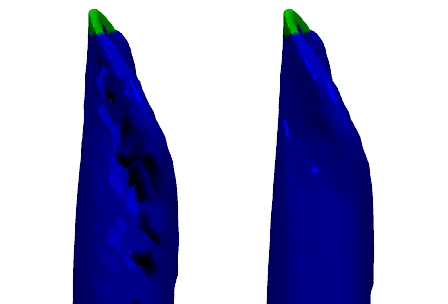
\includegraphics[width=0.5\textwidth]{searchframe.png}
	\caption{Detail reconstruction using the local frame of each vertex (left) and the frame with the shortest displacement vector in the 4-ring neighbourhood (right). }
	\label{fig:searchRing}
\end{figure}

\section{Results}
To evaluate the usability of our tool, we measure the performance for both modifications to the mesh and parameter changes of the operator.
Times are measured on a i5-6600k ($4 \times 3.50$GHz) with 16GB DDR4 running Win10 Pro 64bit.
The test scenario consists of a mesh with 125k vertices, with a handle region containing 15k and the support region 35k vertices. \\
First we consider modifications to the mesh. Updating the support vertices takes just $1.6\si{ms}$, adding the details another $21.6\si{ms}$, resulting overall in a smooth framerate for editing.
\begin{table}
	\centering
	\caption{Measurements for updates to the operator.}
	\begin{tabular}{lc}
		parameter & time [ms] \\
		\hline
		order 1 & 276.77 \\
		order 2 & 922.87 \\
		order 3 & 2262.19 \\
		smoothness & 5692.42 \\
		\hline
	\end{tabular}
	\label{tab:order}
\end{table}\\
Parameter changes require recomputing the higher order operator and precomputing \eqref{lsg}. Times for this are recorded in Table~\ref{tab:order}. A higher order significantly increases computation times and so does the switch to the $LU$ solver for smoothness. Still, a wait time of up to 6s makes it possible to just try out different configurations during editing.
\begin{table}
	\centering
	\caption{Measurements for changes to the smoothing.}
	\begin{tabular}{lc}
		parameter & time [ms] \\
		\hline
		details order 1 & 212.81 \\
		details order 2 & 830.77 \\
		details order 3 & 2168.81 \\
		search ring 1 & 89.59 \\
		search ring 5 & 239.42 \\
		search ring 10 & 725.02 \\
		\hline
	\end{tabular}
	\label{tab:smoothing}
\end{table}\\
Similar values are observed for the smoothing-step in Table~\ref{tab:smoothing}.
Considering that the editing already requires a fixed boundary, the extra implicit smoothing is only useful in edge cases where full reconstruction is not feasible due to strongly stretched or compressed areas. Thus, this time can mostly be saved. A larger seach ring however, can be beneficial in both cases. Above a value of $10$, few differences where observed and considering the extra cost of around $\frac{1}{3}$ of a third order operator computation in this case, this option can always be used.

\bibliographystyle{ieeetr}
\bibliography{references}

\end{document}
